\documentclass[UTF8,zihao=5,scheme=chinese]{ctexart}

\newcommand{\UniversityName}{武汉大学}
\newcommand{\CollegeName}{计算机学院}
\newcommand{\MajorName}{计算机科学与技术（雷军班）}
\newcommand{\CourseName}{自动驾驶技术}
\newcommand{\ReportTitle}{自动驾驶技术第二次实验报告}
\newcommand{\ReportSubtitle}{PETR 六相机三维目标检测}
\newcommand{\StudentName}{尹玉文东}
\newcommand{\StudentID}{2024302131025}
\newcommand{\InstructorName}{张红娟}
\newcommand{\CompletionDate}{2026年9月28日}
\usepackage{../template/course-report}

\begin{document}
\makecoursecover
\tableofcontents
\clearpage

\section{实验概述}

本次实验按课程 PETR 指导文档，使用 nuScenes mini 的六路相机图像完成三维目标检测。
课程代码包提供预处理、训练和测试入口，以及 PETR 模型与 MMDetection3D 底层代码。
我在本机建立独立环境，核对数据和相机几何，运行 20 轮训练，随后在官方 mini\_val
上评估并查看六相机与俯视图。由于预测框偏差明显，我又从第 20 轮权重续训到第 40 轮
进行对照。文中路径均从随报告提交的源代码根目录起算。

\section{实验环境与数据准备}

\subsection{运行环境}

实验在 WSL2 Ubuntu 和 NVIDIA GeForce RTX 4060（8 GB）上运行。Stage 02 使用独立的
Python 3.8.19 环境，主要依赖见表~\ref{tab:environment}。MMCV 的 DCNv2 GPU 前向与反向
计算，以及 PETR 插件导入，均通过了 \path{petr_workflow/environment/check_environment.py}。
本机运行 GPU 脚本时，在命令的 \texttt{LD\_LIBRARY\_PATH} 中临时加入
\path{/usr/lib/wsl/lib}，使 CUDA 库能够找到 WSL 的驱动接口。

\begin{table}[htbp]
  \centering
  \caption{Stage 02 主要环境版本}
  \label{tab:environment}
  \begin{tabular}{ll}
    \toprule
    项目 & 版本 \\
    \midrule
    Python & 3.8.19 \\
    PyTorch / torchvision & 1.13.1+cu117 / 0.14.1+cu117 \\
    MMCV / MMDetection & 1.7.0 / 2.28.2 \\
    MMDetection3D / MMSegmentation & 1.0.0rc6 / 0.30.0 \\
    nuScenes DevKit & 1.1.10 \\
    \bottomrule
  \end{tabular}
\end{table}

\subsection{预处理和数据核对}

原始数据位于 \path{data/nuscenes_mini/}，ResNet50 骨干预训练权重位于
\path{data/petr_assets/}。这次训练只读取相机图像；预处理仍使用 LiDAR 标定和车辆位姿
元数据，将三维标注与相机几何放到同一坐标关系中，不读取 LiDAR 点云。

运行课程入口 \path{petr_workflow/preprocess.py} 后，生成
\path{data/nuscenes_mini/nuscenes_mini_infos_train.pkl} 和
\path{data/nuscenes_mini/nuscenes_mini_infos_val.pkl}。程序检查得到 323 帧训练、81 帧验证，
两组样本没有重复，每帧均关联六张存在的相机图片。它们按官方 mini\_train 和 mini\_val
场景划分，不是随机拆分连续帧。

我还抽取验证样本，比较预处理标注与 nuScenes 原始三维框：位置、尺寸和朝向一致。
将同一标注经过模型框格式和评估转换再映射回全局坐标，位置误差约为
$10^{-6}$ m，尺寸误差约为 $10^{-8}$ m；三维中心通过配置中的相机矩阵投影，
与 DevKit 相机坐标投影的像素误差在数值精度内。

\section{PETR 模型与代码理解}

\subsection{模型和配置}

PETR~\cite{petr} 以六路相机图像为输入。ResNet50 提取图像特征，特征金字塔融合多尺度
信息；位置编码结合相机内外参，将图像特征关联到三维空间，Transformer 查询输出
类别和三维框。本次使用课程的
\path{petr_workflow/PETR-official/projects/configs/teaching/petr_mini_r50.py}，主要设置见
表~\ref{tab:config}。检测头从随机参数开始训练，公开权重只初始化 ResNet50 骨干。

\begin{table}[htbp]
  \centering
  \caption{PETR mini 训练设置}
  \label{tab:config}
  \begin{tabular}{ll}
    \toprule
    参数 & 设置 \\
    \midrule
    相机数量 & 6 \\
    图像尺寸 & $192\times512$ \\
    每卡 batch & 1 \\
    查询数 / 解码器层数 & 100 / 3 \\
    深度采样数 & 32 \\
    优化器初始学习率 & AdamW，$2\times10^{-4}$ \\
    数值精度 & FP32 \\
    \bottomrule
  \end{tabular}
\end{table}

\subsection{代码理解：从相机特征到三维查询}

我重点阅读了检测头
\path{petr_workflow/PETR-official/projects/mmdet3d_plugin/models/dense_heads/petr_head.py}
和 Transformer 实现。检测头先为每个相机特征图的像素位置构造一组深度采样点，再用
\texttt{lidar2img} 的逆矩阵把它们变换到统一的车体（LiDAR）坐标系，并按
\texttt{point\_cloud\_range} 归一化。越界点会写入 mask，不参与后续注意力计算。核心步骤
可概括为：

\begin{minted}[fontsize=\small]{python}
coords = torch.stack(torch.meshgrid([coords_w, coords_h, coords_d]))
coords = torch.cat((coords, torch.ones_like(coords[..., :1])), -1)
coords3d = torch.matmul(img2lidars, coords).squeeze(-1)[..., :3]
coords3d[..., 0:1] = (
    coords3d[..., 0:1] - self.position_range[0]
) / (self.position_range[3] - self.position_range[0])
coords3d[..., 1:2] = (
    coords3d[..., 1:2] - self.position_range[1]
) / (self.position_range[4] - self.position_range[1])
coords3d[..., 2:3] = (
    coords3d[..., 2:3] - self.position_range[2]
) / (self.position_range[5] - self.position_range[2])
coords_position_embedding = self.position_encoder(inverse_sigmoid(coords3d))
\end{minted}

随后，\texttt{reference\_points} 为每个 object query 提供三维参考位置，查询向量与
位置编码一起送入 Transformer decoder。每一层 decoder 的输出分别经过分类分支和回归分支，
回归结果再加回参考点并解码成中心、尺寸、方向和速度。这个实现说明 PETR 的关键不是把六张
图片简单拼接，而是用相机标定把各视角特征放到同一个三维坐标关系中，再由查询完成目标级
聚合；本次生成的六相机投影图和 BEV 图也都使用这一统一坐标关系。

\section{PETR 训练过程}

\subsection{训练设置与日志}

我运行课程入口 \path{petr_workflow/train.py}，训练 20 轮，输出目录为
\path{petr_workflow/outputs/20260928_180737_petr_mini_r50/}。第 20 轮权重为
\texttt{epoch\_20.pth}。训练日志每 10 个 batch 记录一次损失；同轮日志记录的
平均总损失从第 1 轮的 13.415 降到第 20 轮的 8.656。原始文本日志和逐 batch JSON 日志
分别为该目录中的 \texttt{20260928\_180804.log} 和
\texttt{20260928\_180804.log.json}。例如第 20 轮第 320 个 batch 记录的总损失为 9.8336，
分类损失为 0.6761，边界框损失为 2.5828；单个 batch 的损失有波动，表~\ref{tab:loss-log}
按 epoch 汇总的平均总损失更适合观察整体变化。

\begin{table}[htbp]
  \centering
  \caption{训练日志中的代表性轮次}
  \label{tab:loss-log}
  \begin{tabular}{rrr}
    \toprule
    Epoch & 平均总损失 & 运行阶段 \\
    \midrule
    1 & 13.415 & 初始训练 \\
    10 & 9.396 & 初始训练 \\
    20 & 8.656 & 初始训练结束 \\
    21 & 8.804 & 恢复训练 \\
    30 & 8.232 & 恢复训练 \\
    40 & 8.087 & 恢复训练结束 \\
    \bottomrule
  \end{tabular}
\end{table}

为观察继续训练后的变化，我使用 \texttt{--resume-from} 从该权重恢复，并把目标总轮数设为
40，结果单独保存在
\path{petr_workflow/outputs/20260928_194716_petr_mini_r50_resume40/}。
由于总轮数改变，余弦学习率计划也随之改变；恢复日志中第 21 轮学习率约为
$1.0\times10^{-4}$，与 20 轮运行结束时不同。因此这是恢复训练的对照结果，不是严格控制
学习率计划的轮数消融。图~\ref{fig:loss} 标出恢复点。

\begin{figure}[htbp]
  \centering
  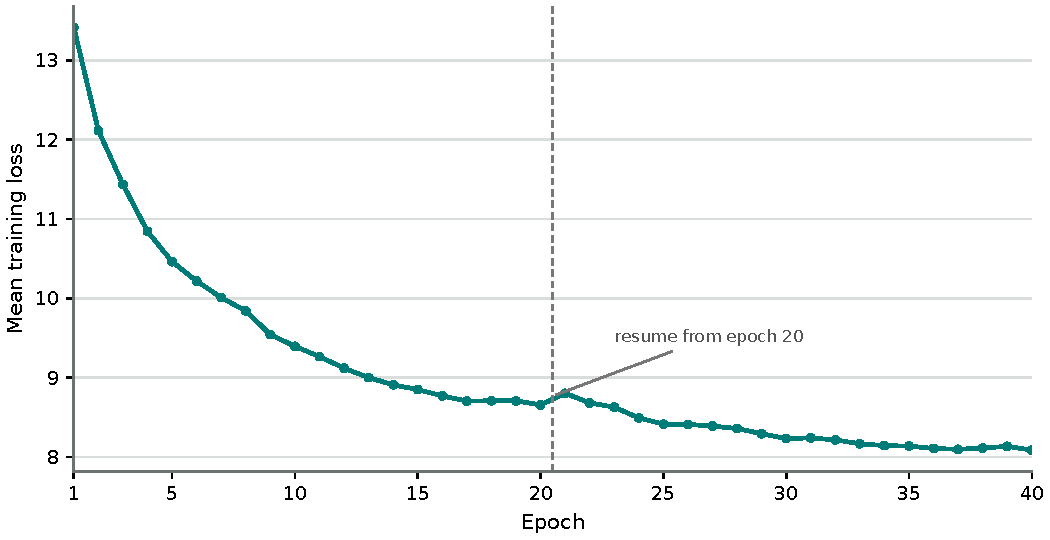
\includegraphics[width=0.85\linewidth]{figures/training_loss.pdf}
  \caption{20 轮训练及续训至 40 轮的平均总损失}
  \label{fig:loss}
\end{figure}
\FloatBarrier

\section{模型测试与结果分析}

\subsection{官方指标}

使用课程入口 \path{petr_workflow/test.py} 分别加载第 20 轮和第 40 轮权重，
在同一 81 帧 mini\_val 上推理，由 nuScenes 官方评估器计算三维目标检测指标。
mini 没有独立的带标注测试集，因此这里的“测试”实际是验证集评估。
表~\ref{tab:metrics} 的数值来自各自 \texttt{test/eval/pts\_bbox/metrics\_summary.json}。

\begin{table}[htbp]
  \centering
  \caption{两个权重在 mini\_val 上的检测结果}
  \label{tab:metrics}
  \begin{tabular}{lrrr}
    \toprule
    权重 & mAP & NDS & car AP \\
    \midrule
    第 20 轮 & 0.000102 & 0.02563 & 0.001016 \\
    第 40 轮 & 0.000082 & 0.02280 & 0.000817 \\
    \bottomrule
  \end{tabular}
\end{table}

两个结果的检测指标均很低，第 40 轮也没有优于第 20 轮。20 轮模型生成了
81 帧的预测文件，包含 6,781 个原始预测框；按类别统计以 car、pedestrian 和 barrier
为主，其他类别没有输出。额外轮数降低了训练损失，但未改善验证指标。

\subsection{六路相机与统一坐标系显示}

\path{petr_workflow/test.py} 使用同一份预测 JSON 绘制三帧对比图。图~\ref{fig:cameras}
上两排是绿色真实框，下两排是红色预测框；六个相机顺序相同。展示时只取分数至少为
0.1 的前 20 个预测框，该阈值只影响图片，不改变表~\ref{tab:metrics} 的评估结果。
六个视角的框先由模型坐标转换到各自相机坐标，再用对应内参投影到图像；因此六路图中的
三维框来自同一车体坐标系，而不是分别在六张图上独立检测。随后将相同的框画到车体坐标系
的 BEV 平面，形成图~\ref{fig:bev} 的统一俯视对照。

\begin{figure}[htbp]
  \centering
  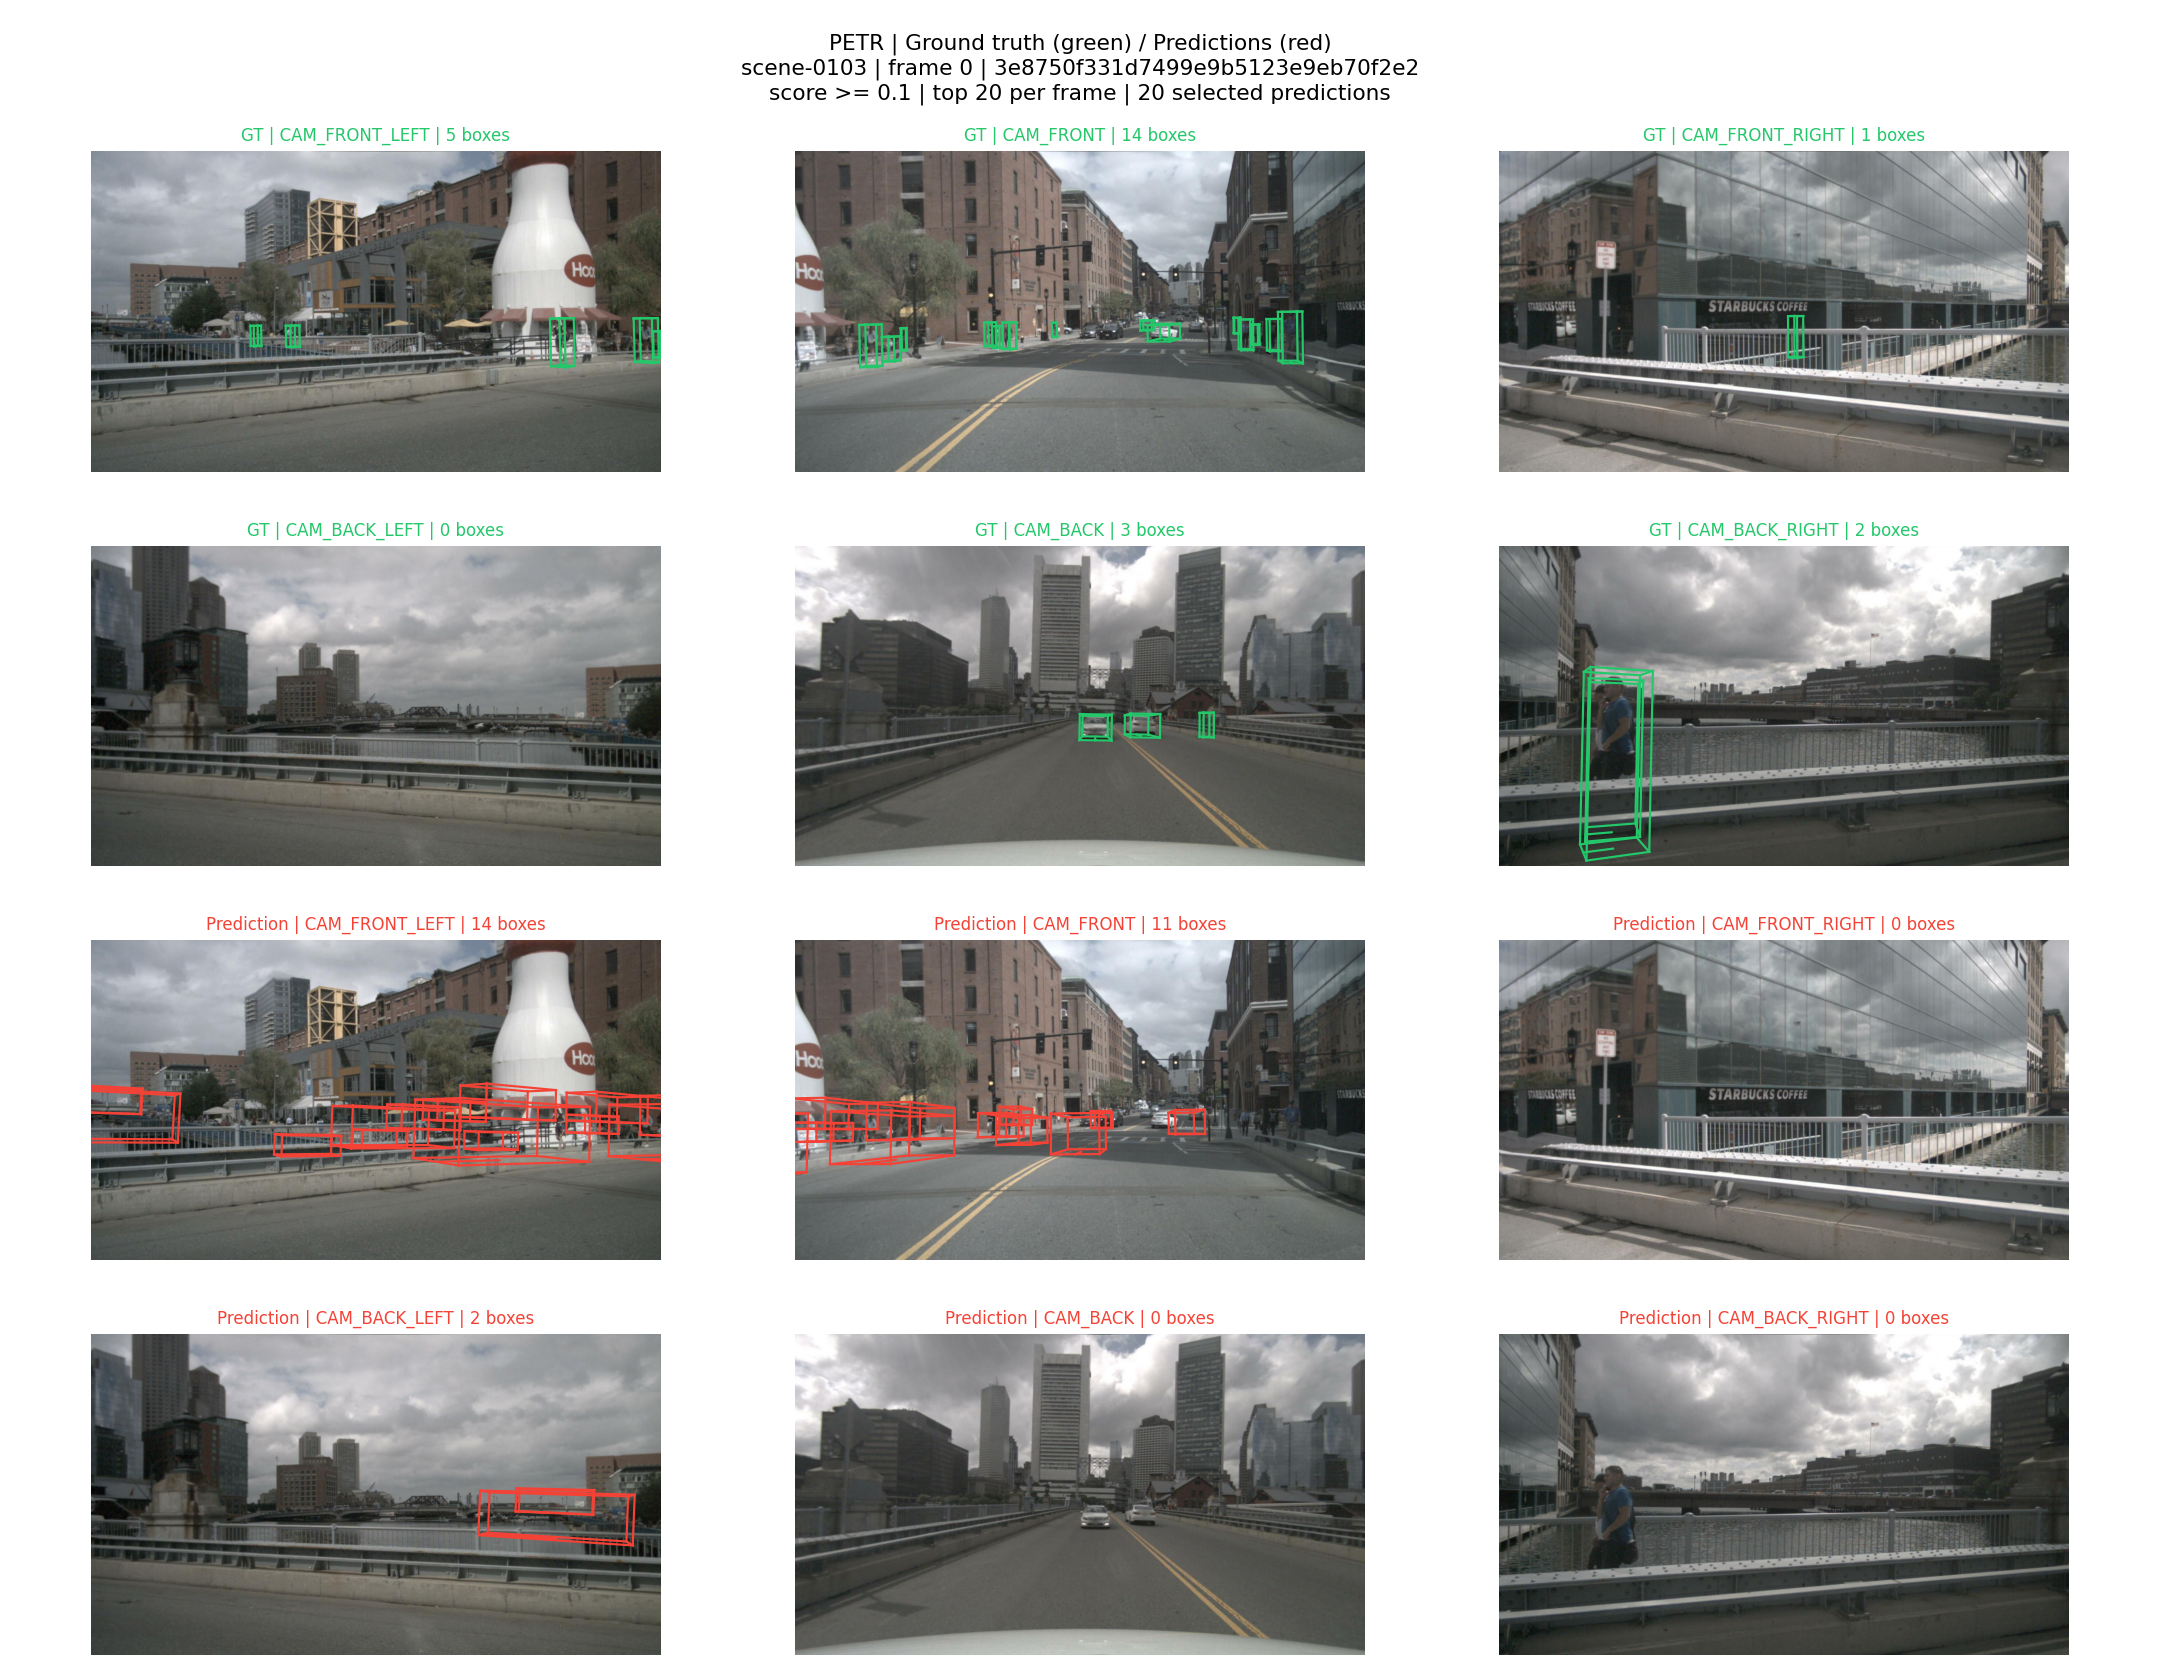
\includegraphics[width=\linewidth]{figures/petr20_scene0103_cameras.png}
  \caption{第 20 轮模型在 scene-0103 一帧上的六相机真实框与预测框}
  \label{fig:cameras}
\end{figure}
\FloatBarrier

图~\ref{fig:bev} 把同一帧的真实框和预测框放在自车坐标系俯视图中。横轴指向车前方，
纵轴指向车左侧，蓝点是车辆原点。第 20 轮的红框主要落在右前方，和绿色真实框
只有少量接近；续训到第 40 轮后，红框大多移至左侧，也没有贴合真实目标。

\begin{figure}[htbp]
  \centering
  \begin{subfigure}[t]{0.48\linewidth}
    \centering
    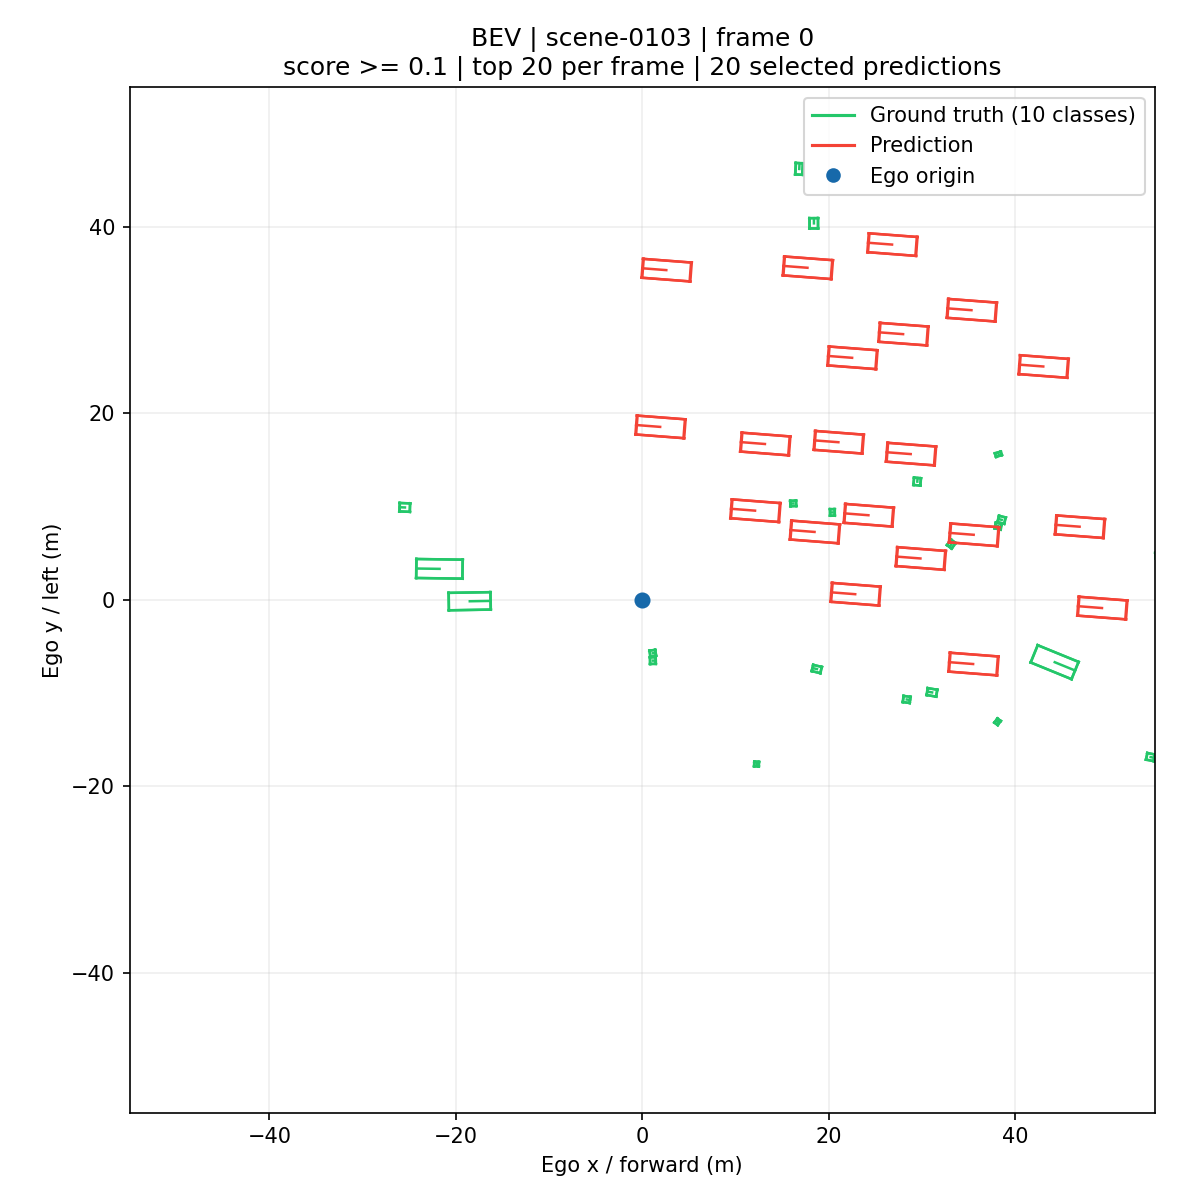
\includegraphics[width=\linewidth]{figures/petr20_scene0103_bev.png}
    \caption{第 20 轮}
  \end{subfigure}
  \hfill
  \begin{subfigure}[t]{0.48\linewidth}
    \centering
    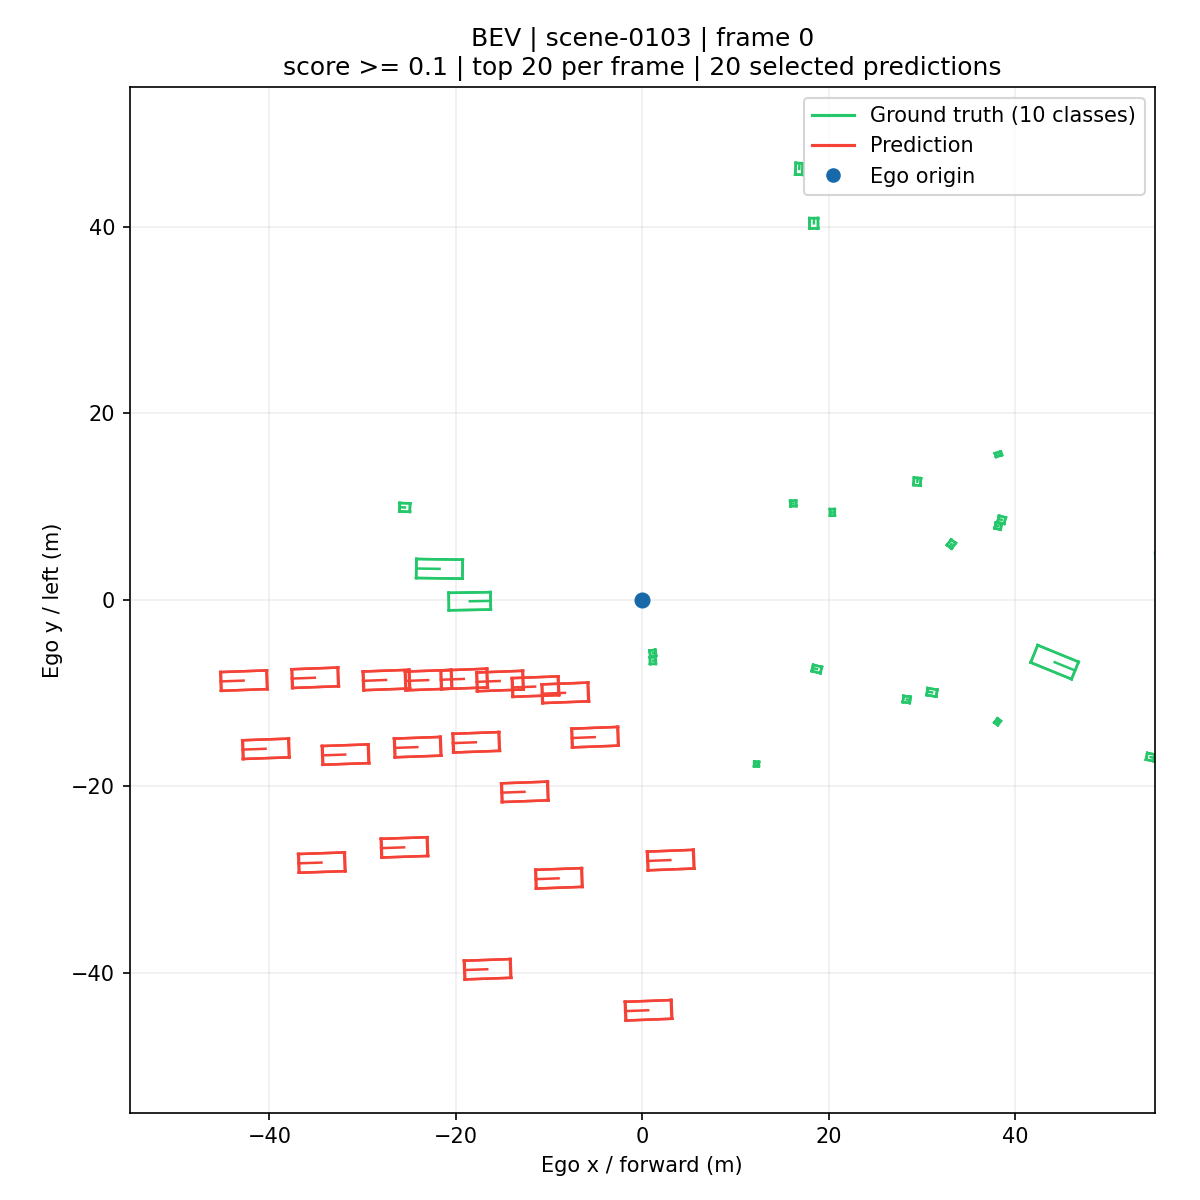
\includegraphics[width=\linewidth]{figures/petr40_scene0103_bev.png}
    \caption{第 40 轮}
  \end{subfigure}
  \caption{同一 mini\_val 帧的三维框俯视图对比}
  \label{fig:bev}
\end{figure}
\FloatBarrier

\section{实验中遇到的问题}

\subsection{检测效果与已有权重}

本次指标和可视化都显示检测效果很差：20 轮的 mAP 为 0.000102、NDS 为 0.02563，
六相机图和 BEV 图中的预测框大多没有贴合真实目标。继续恢复训练到 40 轮后，训练损失
继续下降，但 mAP 降至 0.000082、NDS 降至 0.02280，检测效果没有改善。

我查阅了 PETR 官方仓库的预训练模型信息。官方 PETR-R50-P4 权重是在完整 nuScenes 上
训练的，配置为 $1408\times512$ 输入、900 个 query 和 6 层 decoder，官方训练记录使用
8 张 2080 Ti~\cite{petr-code}。本次课程配置则是 $192\times512$ 输入、100 个 query 和
3 层 decoder，运行环境为单张 8 GB RTX 4060。更关键的是，课程配置文件注明旧版 PETR
完整检测权重不能直接加载；它只提供 ResNet50 骨干权重，并针对当前 MMDetection3D
框约定适配了数据和坐标转换。完整权重包含不同尺寸的 query 与 decoder 参数，直接作为
当前模型权重会遇到结构不匹配；若使用，需切换回官方模型配置并处理版本、数据接口和显存
设置，再单独验证加载与推理。因此我没有把该完整权重接入本次课程实验，也没有声称它已在
本机测试。完整权重更适合作为后续迁移学习实验，不是当前课程流程可直接替换的文件。

\section{实验总结}

数据划分、图片存在性、预处理三维框和相机投影均已核对，训练及官方评估流程也正常完成。
当前检测头仅用 323 帧训练，输入图像缩至 $192\times512$，而模型需要从六路图像学习
三维位置和类别。训练集推理的定位同样不稳定，不能把低指标只归因于验证场景变化。
本次完成了 323/81 帧预处理、20 轮训练、mini\_val 评估和六相机可视化，也检查了 PETR
检测头的坐标位置编码与 Transformer 查询过程。最终结果确实很差；报告如实保留低指标和
预测框偏差。课程包没有提供完整 PETR 检测权重，官方完整权重与教学配置也不能直接对应，
所以本次止于课程规定的训练与评估流程，没有把未验证的权重适配当作实验结果。

\begin{thebibliography}{9}
  \bibitem{petr} Y. Liu et al., ``PETR: Position Embedding Transformation for
  Multi-View 3D Object Detection,'' \textit{ECCV}, 2022.
  \bibitem{nuscenes} H. Caesar et al., ``nuScenes: A Multimodal Dataset for
  Autonomous Driving,'' \textit{CVPR}, 2020.
  \bibitem{petr-code} Megvii Research, ``PETR: Official Implementation and
  Model Zoo,'' \url{https://github.com/megvii-research/PETR}.
\end{thebibliography}

\end{document}
